\documentclass[12pt]{amsart}
\usepackage[pdftex,colorlinks,citecolor=blue,urlcolor=blue]{hyperref}
\usepackage{amssymb}
\usepackage{graphicx,color}
\usepackage{amsmath}
\usepackage{amssymb}
\usepackage{tikz}
\usetikzlibrary{decorations.pathreplacing,calc}

\begin{document}

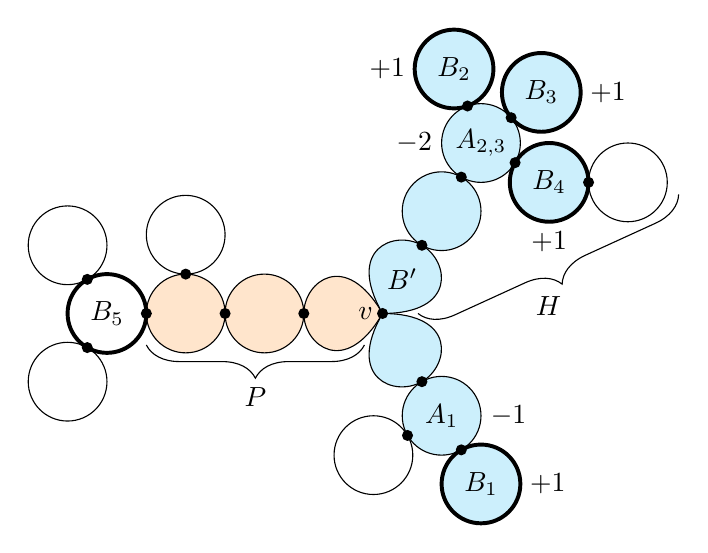
\begin{tikzpicture}
        
        \coordinate (O) at (150:0.5);
        \coordinate (P) at (150:0.5);
        \coordinate (B) at (0.25,0.433);
        \coordinate (C) at (0.25,-0.433);
        
        %Pfad nach links
        \draw[orange!20,thick] (0,0) -- (-1,0);
        \fill[orange!20] (0,0) .. controls (120:0.95) and ($(-1,0)+(90:0.4)$) .. (-1,0);
        \fill[orange!20] (0,0) .. controls (-120:0.95) and ($(-1,0)-(90:0.4)$) .. (-1,0);
        \draw (0,0) .. controls (120:0.95) and ($(-1,0)+(90:0.4)$) .. (-1,0);
        \draw (0,0) .. controls (-120:0.95) and ($(-1,0)-(90:0.4)$) .. (-1,0);
        
        \fill[orange!20] (-1.5,0) circle (0.5);
        \fill[orange!20] (-2.5,0) circle (0.5);
        
        \draw (-1.5,0) circle (0.5);
        \draw (-2.5,0) circle (0.5);
        \draw[line width=0.5mm] (-3.5,0) circle (0.5);
        
        \fill (-1,0) circle (2pt);
        \fill (-2,0) circle (2pt);
        \fill (-3,0) circle (2pt);
        
        \coordinate[label=center:$B_5$] (D) at (-3.5,0);
        
        % zusätzliche Kreise links
        \draw (-2.5,1) circle (0.5);
        \fill (-2.5,0.5) circle (2pt);
        
        \draw ($(-3.5,0)+(120:1)$) circle (0.5);
        \fill ($(-3.5,0)+(120:0.5)$) circle (2pt);
        
        \draw ($(-3.5,0)+(240:1)$) circle (0.5);
        \fill ($(-3.5,0)+(240:0.5)$) circle (2pt);
        
        %Pfad nach oben rechts
        \draw[cyan!20,thick] (0,0) -- ($2*(B)$);
        \fill[cyan!20] (0,0) .. controls (120:0.95) and ($2*(B)+(150:0.4)$) .. ($2*(B)$);
        \fill[cyan!20] (0,0) .. controls (0:0.95) and ($2*(B)-(150:0.4)$) .. ($2*(B)$);
        \draw (0,0) .. controls (120:0.95) and ($2*(B)+(150:0.4)$) .. ($2*(B)$);
        \draw (0,0) .. controls (0:0.95) and ($2*(B)-(150:0.4)$) .. ($2*(B)$);
        
        \fill[cyan!20] ($3*(B)$) circle (0.5);
        \fill[cyan!20] ($5*(B)$) circle (0.5);
        
        \fill ($2*(B)$) circle (2pt);
        \fill ($4*(B)$) circle (2pt);
        
        
        \draw ($3*(B)$) circle (0.5);
        \draw ($5*(B)$) circle (0.5);
        
        
        \coordinate[label=center:$B'$] (K) at (B);
        \coordinate[label=center:$A_{2,3}$] (H) at ($5*(B)$);
        
        
        %zusätzliche Kreise oben rechts
        \fill[cyan!20] ($5*(B)+(40:1)$) circle (0.5);
        \draw[line width=0.5mm] ($5*(B)+(40:1)$) circle (0.5);
        \fill ($5*(B)+(40:0.5)$) circle (2pt);
        \coordinate[label=center:$B_3$] (G) at ($5*(B)+(40:1)$);
        
        \fill[cyan!20] ($5*(B)+(330:1)$) circle (0.5);
        \draw[line width=0.5mm] ($5*(B)+(330:1)$) circle (0.5);
        \fill ($5*(B)+(330:0.5)$) circle (2pt);
        \coordinate[label=center:$B_4$] (I) at ($5*(B)+(330:1)$);
        
        \fill[cyan!20] ($5*(B)+(110:1)$) circle (0.5);
        \draw[line width=0.5mm] ($5*(B)+(110:1)$) circle (0.5);
        \fill ($5*(B)+(110:0.5)$) circle (2pt);
        \coordinate[label=center:$B_2$] (J) at ($5*(B)+(110:1)$);
        
        \draw ($(I)+(1,0)$) circle (0.5);
        \fill ($(I)+(0.5,0)$) circle (2pt);
        
        \coordinate[label=left:$-2$] (M) at ($5*(B)-(0.5,0)$);
        \coordinate[label=left:$+1$] (N) at ($(J)+(-0.5,0)$);
        \coordinate[label=right:$+1$] (O) at ($(G)+(0.5,0)$);
        \coordinate[label=below:$+1$] (P) at ($(I)+(0,-0.5)$);
        
        %Pfad nach unten rechts
        \draw[cyan!20,thick] (0,0) -- ($2*(C)$);
        \fill[cyan!20] (0,0) .. controls (0:0.95) and ($2*(C)-(210:0.4)$) .. ($2*(C)$);
        \fill[cyan!20] (0,0) .. controls (240:0.95) and ($2*(C)+(210:0.4)$) .. ($2*(C)$);
        \draw (0,0) .. controls (0:0.95) and ($2*(C)-(210:0.4)$) .. ($2*(C)$);
        \draw (0,0) .. controls (240:0.95) and ($2*(C)+(210:0.4)$) .. ($2*(C)$);
        
        \fill[cyan!20] ($3*(C)$) circle (0.5);
        \draw ($3*(C)$) circle (0.5);
        \fill[cyan!20] ($5*(C)$) circle (0.5);
        \draw[line width=0.5mm] ($5*(C)$) circle (0.5);
        
        \fill ($2*(C)$) circle (2pt);
        \fill ($4*(C)$) circle (2pt);
        \fill ($3*(C)+(210:0.5)$) circle (2pt);
        
        \draw ($3*(C)+(210:1)$) circle (0.5);
        
        \coordinate[label=center:$A_1$] (F) at ($3*(C)$);
        \coordinate[label=center:$B_1$] (E) at ($5*(C)$);
        
        \coordinate[label=right:$-1$] (L) at ($3*(C)+(0.5,0)$);
        \coordinate[label=right:$+1$] (L) at ($5*(C)+(0.5,0)$);
        
        \coordinate[label=left:$v$] (A) at (0,0);
        \fill (A) circle (2pt);
        
        %geschweifte Klammer
        \draw[decorate,decoration={brace,mirror,amplitude=12pt}] (-3,-0.4) -- (-0.23,-0.4) node[midway, below,yshift=-12pt,]{$P$};
        \draw[decorate,decoration={brace,mirror,amplitude=12pt}] (0.45,0) -- ($(I)+(1.65,-0.15)$) node[midway, below,yshift=-12pt,]{$H$};
    \end{tikzpicture}

\end{document}